\documentclass[mastersthesis,12pt]{wuthesis}     %% LaTeX2e document.
%
% Use one of the following
% \documentclass[mastersthesis,12pt]{wuthesis}
% \documentclass[dscthesis,12pt]{wuthesis}
% \documentclass[phdthesis,12pt]{wuthesis}
%
% If you want to use other packages such as amstex, or epsfig
% \usepackage them here.
%
% epsfig, ellipsis, and caption are 'packages' for LaTeX2e and
% should be part of your distribution.  If not talk to your
% sysadmin
\usepackage{epsfig}
\usepackage{ellipsis}
\usepackage[center]{caption}
%%%%%%%%%%%%%%%%%%%%%%%%%%%%%%%%%%%%%%%%%%%%%%%%%%%%%%%%%%%%%%%%%%%%%%%%%%%%%
%%
%% These commands customize the `wuthesis' package for me
%%
%%%%%%%%%%%%%%%%%%%%%%%%%%%%%%%%%%%%%%%%%%%%%%%%%%%%%%%%%%%%%%%%%%%%%%%%%%%%%

%% Enter your official name
\renewcommand{\thesisauthor}{Richard Speyer}
\renewcommand{\thesisauthorlastname}{Speyer}

%% Enter your previous degrees
%% If you have no previous degrees remember to remove the comma too.
%\renewcommand{\thesisauthorpreviousdegrees}{, J.D.}

%% Enter department name
\renewcommand{\thesisdepartment}{Department of Computer Science and Engineering}
\renewcommand{\thesisfield}{Computer Science}

%% Enter date of graduation
\renewcommand{\thesismonth}{May}
\renewcommand{\thesisyear}{2009}

%% Enter title of thesis
\renewcommand{\thesistitle}{Using Regression Techniques to Correllate Weather Signals with Image Sequences}
\renewcommand{\thesisshorttitle}{Learning to Find Signals in Image Sequences}

%% Enter the copyright holder ( DEFAULT is \thesisauthor )
%\renewcommand{\thesiscopyrightholder}{\thesisauthor}

%% Enter supervisor name
\renewcommand{\thesissupervisor}{Professor Robert Pless}
\renewcommand{\thesiscommittee}{Robert Pless \\
	William Smart \\
	Ron Cytron}

%% Enter the dedication
% \renewcommand{\thesisdedication}{Dedicated to my parents.}

%%%%%%%%%%%%%%%%%%%%%%%%%%%%%%%%%%%%%%%%%%%%%%%%%%%%%%%%%%%%%%%%%%%%%%%%%%%%%
%%
%% This paper is construced from other files.  Each \include'd file
%% begins a chapter.  This is done for easy developement and revision.
%%
%%%%%%%%%%%%%%%%%%%%%%%%%%%%%%%%%%%%%%%%%%%%%%%%%%%%%%%%%%%%%%%%%%%%%%%%%%%%%

\begin{document}

\frontmatter
%%
%  This is all that frontmatter stuff
%
%  This way I can 'not' include it easily

% NOTE: do not put any text in the thesistitlepage, thesiscopyrightpage,
% or thesisdedicationpage sections.  If you want to use these pages, then you
% should remove the notes below (e.g., by uncommenting the \iffalse
% and \fi lines) and change the appropriate fields in thesis-main.tex.
% This will ensure that the copyright and dedication lines are positioned
% and formatted correctly.  Additionally, remove the
% thesisacknowledgmentpostscript and listoftablespostscript sections, since
% these are used to add explanatory notes which shouldn't be there in normal
% theses.

\begin{thesistitlepage}               %% Generate the title page.
\iffalse
\begin{singlespace}
\tiny
{\small \textbf{How to use this document:}}
This sample document outlines guidelines for the proper formatting of theses
and dissertations for Master's and D.Sc.\ degree seeking students within the
School of Engineering at Washington University.  (Ph.D.\ students can also make
use of this document; see special note below.)  This document is formatted
using the same guidelines which it describes.  Consequently, by making an extra
copy of this document you can use it as a template into which you can insert
your own thesis or dissertation textual matter, replacing the original text
with your own while still retaining the general formatting contained within.
This document/template can be downloaded (as either a Microsoft WORD document
OR as a set of \LaTeX{} files) from the Engineering Student Services' web site
and is located with other engineering graduate forms and guides.

{\small \textbf{Important reminders of what needs to be updated:}}
Be certain to use your own full name wherever appropriate.  After removing
these comments, be sure to vertically center the information on this title page
to assure an equal amount of ``white space'' exists both above and below your
title page information.  Your examination committee will likely contain only
three members if you are a Master�s student, as shown in the sample above.
However, D.Sc.\ committees will typically have five members, and Ph.D.\
committees will have six.  Make sure you use the month and year your degree is
officially to be \uline{earned} on the title page, abstract page, and on any
vita page included.  \uline{If this is for your doctoral degree (i.e., either
D.Sc.\ or Ph.D.),} be sure to change all occurrences of the word ``thesis'' to
display as ``dissertation'', and change ``MASTER OF SCIENCE'' to ``DOCTOR OF
SCIENCE'' or ``DOCTOR OF PHILOSOPHY'', whichever applies.   \uline{IMPORTANT:
If you are a Ph.D.\ student,} you must also change the line above (near the
midsection of this page) to ``A dissertation presented to the Graduate School
of Arts and Sciences'' (but do NOT change the reference to the ``School of
Engineering'' which is at the very top of this page, as that must be left
exactly as shown.

{\small \textbf{Note for Ph.D.\ Students:}}
The formatting contained within this sample document can serve well in
emulating the basic formatting needed for the Ph.D.\ dissertation.   However,
please remember that all Ph.D.\ students are ultimately responsible for meeting
the Graduate School of Arts \& Sciences' formatting guidelines.  The GSAS
dissertation guidelines are published on the Graduate School web site located
with other documentation for GSAS policies and guides.  Be sure to read
``Important reminders'' in paragraph above.
\end{singlespace}
\fi
\end{thesistitlepage}

\iffalse
\begin{thesiscopyrightpage}                 %% Generate the copyright page.
\begin{singlespace}
\scriptsize
{\small \textbf{Important Notes Regarding Copyright Option:}} \\
Technically, a thesis or dissertation is protected to some degree by copyright
laws with or without a student having to register his or her claim to
copyright.  However, including a copyright page and applying for registration
of ones claim to copyright provide extra measures of legal protection from
potential copyright infringement.  There is a fee connected with explicitly
registering to copyright ones work; because of this, many students do not
choose to register to copyright their work.  Students should check with their
advisor(s) and/or seek legal advice to gather further information helpful to
making a decision with regards to registering their claim to copyright.  If you
are \uline{not} going to register to copyright your work, then you can choose
to remove this page from your document.  However, if you do choose to
explicitly copyright your work, then leave this page in, change the name to
your name, change the year to the appropriate year in which your degree will be
earned, and remove these notes of informational text.  If a student wishes to
officially ``register'' this claim to copyright, then Masters students will
need to pursue that effort on their own and can find appropriate options by
searching the web; Doctoral students can complete an authorization to apply for
registration (i.e., of their claim to copyright the dissertation) by indicating
this interest in the appropriate area of the UMI Dissertation Publishing
Agreement Form (i.e., on the form which they will submit along with their final
dissertation material) available from the Engineering Student Services web
site.

{\small \textbf{Important Notes Regarding Page Numbering and Margins:}} \\
If you decide to include this copyright page in your final document, do
\uline{not} count the page among your counted pages, and do \uline{not} display
any page number on the page.  \uline{Every sheet of paper in the manuscript
should be numbered except for two:  the title page and this optional copyright
page.}Specifically, the front textual information (which comes before your main
thesis/dissertation body of text) is numbered with Roman numerals, and your
main body of text begins with Arabic numbers.  Since the title page is counted
but \uline{not} numbered, roman numeral \uline{``ii'' is always the first
number used and appears on the page AFTER the title page (AND AFTER the
copyright page, IF included)} --- as shown in this sample template document.
Page numerals should always display centered, just above the 1 bottom margin.
The left margin should be 1.5 inches, with a 1 inch margin at top, bottom, and
right.  The left margin is extra-wide in order to accommodate the binding
process.  When typing the manuscript, stay well within these margin guides.
Lastly, remember to update your table of contents such that the page numerals
referenced there will match the page numbers on the bottom of the pages to
which they make reference in your document.  This is necessary to do manually
because, unfortunately, the page numbering within this templates table of
contents is \uline{not} automatically linked to the pages of the body of text.
This is further documented, along with some work arounds, in the appendix to
this guide called Special Notes for MS WORD Users.  \LaTeX{} users may have to
invent other solutions with regards to synchronizing table of contents page
references with actual document page numbers.  This guide merely provides a
helpful starting point.  \textbf{REMINDER:} When you remove these comments, be
sure to leave the copyright information centered both vertically and
horizontally on the page.
\end{singlespace}
\end{thesiscopyrightpage}
\fi

\begin{thesisabstract}
\textbf{Reminders of what needs to be updated:}
After removing these comments, begin typing the body of your abstract here,
\uline{double-spaced}.  It is acceptable if the body of the abstract continues
onto the next page (as in this sample abstract), but \uline{the body of the
abstract is limited to a maximum of 350 words (excluding the heading
information listed above).  NOTE: This sample abstract is too long, as it
exceeds 350 words.}  The point-size of the body of the abstract can be set to
12 point (which is the text size of this sample comment-paragraph) or it can be
reduced to 10 point if you prefer.  Regardless of which specific point size you
select, the abstract must remain double-spaced and it should \uline{not} be
bolded.  \uline{If this is for your doctoral degree, be sure to change all
occurrences of the word ``thesis'' to display as ``dissertation'', and change
``Master of Science'' to ``Doctor of Science'' or ``Doctor of Philosophy'',
whichever applies.}  In the abstract heading above, make sure you \uline{use
the year your degree is officially to be earned}.  Be sure to use your full
name and your research advisor�s full name wherever appropriate, and be certain
to use the correct title of your degree whenever referencing it. The title of
your degree will not always be the same as the title of your department or
program, so please check with your departmental administrative assistant and
advisor(s) to be sure you are using the correct degree title.  Questions you
may have about preparing your theses or dissertations are always welcomed at
the Office of Engineering Student Services.

\textbf{Note for Ph.D.\ Students:}
The formatting contained within this sample document can serve well in
emulating the basic formatting needed for the Ph.D.\ dissertation.   However,
please remember that all Ph.D.\ students are ultimately responsible for meeting
the Graduate School of Arts \& Sciences' formatting guidelines.  The GSAS
thesis and dissertation guidelines are published on the Graduate School web
site located with other documentation for GSAS policies and guides.  Be sure to
read all of the above notes/reminders on what needs to be updated as shown in
this template document�s title, copyright, and abstract pages.  Ph.D.\ students
will submit final dissertations and all materials to the Office of Graduate
School of Arts and Sciences, and any questions about their dissertations should
also be directed to that office.
\end{thesisabstract}

%\iffalse
\renewcommand{\thesisacknowledgmentpostscript}{
\textbf{Reminders of what needs to be updated:}
After removing these comments, use the above format to help input your
acknowledgments page.   A special dedication can be placed as the final
paragraph, as shown above; alternatively, you may include a special dedication
on the page that follows, as also shown in this sample template.}
%\fi

\begin{thesisacknowledgments}
An acknowledgments page should be included in your final thesis or
dissertation.  In the final copy, it should be placed immediately before the
table of contents.  If you wish to include a special dedication, then you may
use the dedication to close the acknowledgments page or place it on the page
that immediately follows the acknowledgments page.  

It is appropriate to acknowledge sources of academic and financial support;
some fellowships and grants require acknowledgment.  Consequently, I would like
to thank the Dean for having the foresight and vision necessary to understand
the importance of funding the development of this sample thesis/dissertation
template.

A special thanks goes to the many graduate students and distinguished faculty
within my department who have reviewed this thesis and helped support the
related research.
\end{thesisacknowledgments}

\iffalse
\begin{thesisdedicationpage}                %% Generate the dedication page.
\textbf{Note:} You may include a special dedication as shown here.  If you
include this page, be sure to keep it brief and center it on the page both
horizontally and vertically.  Alternatively, you may remove this page
altogether, and a special dedication can be placed as the final paragraph to
your acknowledgments page (as shown in this document on the preceeding page).
\end{thesisdedicationpage}
\fi

\begin{singlespace}
\tableofcontents

\iffalse
\renewcommand{\listoftablespostscript}{
\small
\textbf{Note:} Be consistent in aligning multi-lined table-names, figure-names,
and chapter/section-names throughout your document.  It is generally
recommended to make sure any additional lines (i.e., within a long title or a
long table name) wrap and align immediately under the 1st character of the
title or name with which they are associated in the line immediately above ---
as shown in the ``Table 2.1'' example above.   Whatever approach you take, be
consistent.}
\fi

\listoftables

\listoffigures
\end{singlespace}

\iffalse
\chapter{Preface}

This guide contains the School of Engineering's rules for formatting theses and
dissertations.\footnote{Throughout this guide, the word thesis refers to both
theses and dissertations.}   Departments, advisors, and committees may impose
additional rules.  In the past, students were required to study a similar (but
much longer) set of rules and apply them to their theses.  The Association of
Graduate Engineering Students (i.e., AGES) has helped to prepare templates and
style files that simplify thesis preparation.  These files have been set up to
produce acceptably formatted theses and dissertations using several popular
word processing and text formatting programs.  There should be one available in
Microsoft WORD and another in \LaTeX{}.  Students can retrieve these files and
their accompanying instructions from the Engineering Student Services' main web
page.  Check with Engineering Student Servcies (Lopata Hall, Room 303) if you
have any questions.  Students who create their own templates or style files are
invited to submit these files for future use by others.  This guide you are
now reading can be downloaded (in either MS WORD formatted version or a \LaTeX{}
version) and can be utilized as a template for formatting your own theses.  In
short, the margin settings, pagination, table of contents logic, etc. are
already established in the downloadable versions.  You can simply replace the
text within the template with your own text, thereby saving you much setup
time.  \textbf{NOTE:} \uline{This preface page is optional.  A preface page
is usually used to explain further details surrounding the background and
motivation for the work.  You can remove it completely}, but then be sure the
reference to this page is also removed from the Table of Contents.  The
majority of students do not include a preface page.
\fi

%%
%% For List of Abbreviations, Glossary or Nomenclature also
%% use \chapter, but put some kind of list environment inside.



%%% Local Variables: 
%%% mode: latex
%%% TeX-master: "thesis-main"
%%% End: 


\mainmatter
\chapter{Thesis Format}
\label{cpt:format}

The following guidelines offer you some degree of flexibility in formatting
your thesis. Options are summarized in Table~\ref{tab:options}.  Whatever
options you choose to use, you must use them consistently throughout document.

\section{Margins}

Your \underline{printed output} must reflect a \underline{physically
measurable} left margin of at least 1.5 inches, with top, bottom, and right
margins measurable at 1 inch.  Some systems' settings produce varying results
when printing to different printers, so be sure to measure your output.
Remember, nothing (not even page numbers) should print in the margins.

\section{Page Numbers}

Number all pages in your thesis except the title page and the optional
copyright page which might follow the title page.  Number the ``front matter''
pages (i.e., the pages that come prior to the main body of text, prior to
chapter 1) with lowercase Roman numerals, centered immediately above the bottom
margin, and starting with the Roman numeral ``ii''.  Number the pages starting
with the first page of the first chapter with Arabic numerals, also centered
immediately above the bottom margin, and starting with numeral ``1''.

\section{Body Text}

Use a 10, 11, or 12-point Garamond, Times Roman or Times New Roman font for
your thesis text.  {\scriptsize (The MicroSoft WORD based ``template'' uses
Garamond throughout, and is recommended whenever possible.  The \LaTeX{}
version uses a high quality variation of the Times Roman font.  Whichever is
used, be consistent throughout your document..)}  Use 1.5 or double line
spacing for most body text.  Block quotes should be single spaced.  Use either
left justification with a ragged right edge, or full justification.  Paragraphs
may be set in a block style, with no indentation, or they may be indented up to
0.5 inch.  Skip a line between paragraphs.

\section{Titles and Headings}

Titles and headings may be left-justified or centered.  Capitalize the first
letter of the first word and the first letter of each subsequent major word in
a title or heading.  Do not capitalize articles, prepositions, and conjunctions
that are not the first word of a title or heading.  For example, do not
capitalize such words as the following: a, an, the, for, to, on, or.
Formatting specifications for particular types of headings and titles are
described below.  You may use a plain or bold version of the body text font for
all titles and headings.

\subsection{Chapter Titles}

Begin each chapter on a new page.  You may start the chapter title below the
top margin  (1.5 inches from the top edge of the page), or you may leave some
space and start the chapter title up to 3 inches from the top edge of the page.
There are two options for formatting the chapter title:
\begin{itemize}
\item Type the word ``Chapter'' followed by the chapter number, skip a
  line, and type the chapter title on the following line; or
\item Type the chapter number followed by the chapter title, all on
  the same line.
\end{itemize}
You may use a font size of up to 36 points for the chapter title.  

\subsection{Section Headings}

You may use a font size of up to 24 points for the section headings.  Type the
chapter number and section number before the section title.

\subsection{Subsection Headings}

You may use a font size of up to 18 points for subsection headings.  Type the
chapter number, section number, and subsection number before the subsection
title.

\subsection{Headings for Divisions Smaller than Subsections}

Use unnumbered headings for divisions smaller than subsections.  You may use a
font size of up to 14 points.  Headings may be typed above or on the same line
as the sections they label.  You may use both styles within your thesis.

\paragraph{Run-in Headings}
To the left is an example of a run-in heading.  Notice that it is typed on the
same line as the section that it labels.  It may be used for divisions smaller
than subsections.

\begin{figure}[h]
\centering
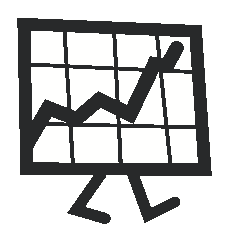
\includegraphics{justafigure}
\caption{Just a Figure\label{fig:justafigure}}
\end{figure}

\section{Figures and Tables}

Figures and tables must be referenced in the text by number.  They must be
numbered consecutively throughout each chapter, with the chapter number
preceding each figure or table number.  For example, the third figure in
chapter 1 would be labeled Figure 1.3.  You may either:
\begin{itemize}
\item Maintain one numbering sequence for figures and another for
  tables, and label figures with the word ``Figure'' and tables with the
  word ``Table''; or
\item Label both figures and tables with the word ``Figure'' and
  maintain one numbering sequence.
\end{itemize}
Place figures and tables as close to their references in the text as
possible.  Place a figure number and title below each figure (or table
labeled as a figure).  Place a table number and title above each table
labeled as a table.  In figures and tables, avoid using color and
avoid text smaller than 10 points.  Do not let figures or tables spill
out into the margins.  Figure~\ref{fig:justafigure} is an example figure.

\section{Lists}

You may include lettered, numbered, or bulleted lists in your thesis.
Use consistent punctuation and capitalization throughout each list.
Lists may be indented.

\section{Footnotes and Endnotes}

You may use footnotes or endnotes for brief notes that are not appropriate for
the body of the text.  Use either footnotes or endnotes consistently throughout
your thesis.  Position footnotes in 10 point type just above the bottom margin
and page number.  Use a short horizontal rule to separate footnotes from the
text.  Position endnotes at the end of each chapter.  Type endnotes using the
same font size and justification as the body text.  Single space within each
footnote or endnote; double-space between footnotes or endnotes.  Footnotes and
endnotes should be consecutively number.

\section{Quotations}

You must use quotation marks and parenthetical references to indicate words
that are not your own. Put quotation marks around short quotes.  Put long
quotes in separate single-spaced paragraphs, indented up to 1 inch from the
left margin (these are called block quotations).  Kate Turabian, editor of
official publications and dissertation secretary at the University of Chicago
for over 25 years, distinguishes short and long quotes as follows:

\begin{quote}
  Short, direct prose quotations should be incorporated into the text
  of the paper and enclosed in double quotation marks: ``One small step
  for man; one giant leap for mankind.'' But in general a prose
  quotation of two or more sentences which at the same time runs to
  four or more lines of text in a paper should be set off from the
  text and indented in its entirety\dots.~\cite{Turabian}
\end{quote}

\section{Equations}

Equations may be set in-line with the text or numbered and placed in separate
paragraphs.  Use the same numbering style for equations as you would for
figures and tables.  Here is an example of an equation set in-line with a
paragraph: $E = mc^2$.  Here is an example equation placed in a separate
paragraph:
\begin{equation}
E = mc^2
\end{equation}
Equation numbering and formatting should follow the usual convention of your
discipline and be acceptable to your thesis committee.

\newpage
\begin{table}[h]
	\caption{Thesis Formatting Options\label{tab:options}}
	\vspace{0.125in}
	\centering
	\hyphenpenalty10000  % turn off hyphenation in this table.  It looks bad.
	
	\begin{tabular*}{\textwidth}{|c|@{\extracolsep{\fill}}c|}
		\hline
		\textbf{Thesis Element} & \textbf{Formatting Options} \\ \hline
		\textbf{title page font} & \small 12-point or 14-point Garamond, Times or Roman \\ \hline
		\textbf{table of contents chapter title} & \small bold or plain \\
			\textbf{font} & \\ \hline
		\textbf{first-level table of contents} & \small 0 to 0.5 inch \\
			\textbf{indentation} & \\ \hline
		\textbf{second-level table of contents} & \small 0 to 1.0 inch \\
			\textbf{indentation} & \\ \hline
		\textbf{body text font} & \small 10, 11, or 12-point Garamond, Times or Roman \\ \hline
		\textbf{body text line spacing} & \small 1.5 or 2 \\ \hline
		\textbf{body text justification} & \small left or full \\ \hline
		\textbf{paragraph indentation} & \small 0 to 0.5 inch \\ \hline
		\textbf{chapter title position} & \small 1.5 to 3 inches below top edge of page \\ \hline
		\textbf{chapter title style} & \small heading preceded by the word ``Chapter'' and \\
			& \small the chapter number or, heading preceded only \\
			& \small by the chapter number \\ \hline
		\textbf{chapter title} & \small 10-pt to 36-pt font, centered or left-justified, \\
			& \small plain or bold \\ \hline
		\textbf{section heading} & \small 10-pt to 36-pt font, centered or left-justified, \\
			& \small plain or bold \\ \hline
		\textbf{subsection heading} & \small 10-pt to 36-pt font, centered or left-justified, \\
			& \small plain or bold \\ \hline
		\textbf{unnumbered headings} & \small 10-pt to 36-pt font, centered or left-justified, \\
			& \small plain or bold \\ \hline
		\textbf{table labels} & \small label tables as ``Table'' or ``Figure'' \\ \hline
		\textbf{Parenthetical reference style} & \small author-date system, numbered, or another style \\
			& \small acceptable to your committee \\ \hline
		\textbf{Reference list style} & any style acceptable to your committee \\ \hline
	\end{tabular*}
\end{table}

%%% Local Variables: 
%%% mode: latex
%%% TeX-master: "thesis-main"
%%% End: 

%
%\addtocontents{toc}{\newpage}
\chapter{Parts of the Thesis}

This chapter describes the components of a thesis.  You need not include all
components described here, but you must follow the prescribed order for the
components you do include. Table~\ref{tab:components} lists the required and
optional components in the order that they should appear.  Your thesis should
include three main parts: the front matter, the text, and the back matter.
Each of these parts is described below.

\section{Front Matter}

The front matter includes all material that appears before the beginning of the
main text.  Number all ``front matter'' pages (except the title page and the
optional copyright page) with lower-case roman numerals, centered just above
the bottom margin.  Each of the following sections should begin on a new page.

\subsection{Title Page}

Format the title page precisely as the title page to this document is
formatted:  include a 1.5-inch left margin, a 1-inch top margin, a 1-inch right
margin, and a 1-inch bottom margin.  Use a 12- or 14-point regular Garamond,
Times or Roman font on this page.  If you are writing a dissertation,
substitute the word ``dissertation'' wherever the word ``thesis'' appears in
this document.  The date on the title page should reflect the month and year
the degree will be awarded and should be one of the following months:
December, May, or August.  Do \uline{not} number the title page.

\begin{table}[ht]
\refstepcounter{table}
\label{tab:components}
\centering
Table \ref{tab:components}: Required and Optional Thesis Components
\addcontentsline{lot}{table}{\numberline{\ref{tab:components}}{%
	\ignorespaces Required and Optional Thesis Components
	(NOTE: If you have a multi-lined table label/title, then the 2nd and
	all additional lines should align with the first line, just like this
	one; plus, be sure that no words display to the far right hand side
	where the page numbers for your tables display, just as shown in this
	example.)}}

% Note: the \addcontentsline is a hack to force LaTeX to add a different
% entry to the text and table-of-contents.  Don't do this normally.

\vspace{0.125in}
\begin{spacing}{1}
\begin{tabular}{| c | c | c | c|}
\hline 
\textbf{Major Part} & \textbf{Thesis Component} & \textbf{Required}
 & \textbf{Optional} \\ \hline

\textbf{Front Matter} & Title Page & $\bullet$ & \\ \cline{2-4}
 & Abstract Page & $\bullet$ & \\ \cline{2-4}
 & Copyright Page & & $\bullet$ \\ \cline{2-4}
 & Dedication & & $\bullet$ \\ \cline{2-4}
 & Table of Contents & $\bullet$ & \\ \cline{2-4}
 & List of Tables & (Rqrd if used) & \\ \cline{2-4}
 & List of Figures & (Rqrd if used) & \\ \cline{2-4}
 & List of Abbreviations & & $\bullet$ \\ \cline{2-4}
 & Glossary of Nomenclature & & $\bullet$ \\ \cline{2-4}
 & Acknowledgments & & $\bullet$ \\ \cline{2-4}
 & Preface & & $\bullet$ \\ \hline

\textbf{Text} & Chapters & & $\bullet$ \\ \hline

\textbf{Back Matter} & Appendices & & $\bullet$ \\ \cline{2-4}
 & References & $\bullet$ & \\ \cline{2-4}
 & Vita & $\bullet$ & \\ \cline{2-4}
 & Short Title Page & $\bullet$ & \\ \hline
\end{tabular}
\end{spacing}
\end{table}

\subsection{Copyright Page}

Include a copyright page if you plan to copyright your thesis.  If used, the
copyright page must be unnumbered, immediately following the title page.  It
should include three lines, centered on the page with regular body text font
and spacing.  The 1$^{st}$ line should be ``copyright by'', the 2$^{nd}$ line
should contain your full name.  The 3$^{rd}$ line should contain the year the
degree is to be awarded.  Do not number the copyright page.  If you are an
Master's candidate and would like to register your claim to copyright your
thesis, you must make all arrangements independently.  Doctoral students will
complete a publishing agreement form which will give them a copyright
registration option.

\subsection{Abstract Page}

The abstract must be 350 words or fewer.  Format the abstract page precisely as
done in this document.  The abstract page \uline{always} begins the document's
page numbering at ``ii''.

\subsection{Acknowledgments}

An acknowledgments section should be included..  Use it to thank those who
supported your research through contributions of time, money, or other
resources.  Type the word ``Acknowledgments'' in chapter title style at the top
of page.  If the acknowledgments fill more than one page, put the heading only
on the first page.  Number the page with a Roman numeral, centered at bottom,
sequentially following the abstract page(s) Roman numeral(s).

\subsection{Dedication}

The dedication page is optional.  If you decide to include a separate
dedication page,  make it short and center it on the page.  If included, you
should number it, placing the next logical/sequential Roman numeral at bottom
of page, centered, as shown in this sample document.

\subsection{Table of Contents}

The table of contents must include the page numbers of all chapters and
sections of your thesis.  In addition, it may include the page numbers of all
subsections.  It must also include the page numbers of all front and back
matter elements, unless otherwise specified.  Chapter titles should appear
flush left, section headings may be indented up to 0.5 inch, and subsection
headings may be indented up to 1 inch.  Chapter titles may be typed in plain or
bold font.  All titles and headings must be followed by a dot leader and a page
number.  The word ``Contents'' must appear in chapter title style at the top of
the page.  Be sure to align multi-lined chapter titles in the table of
contents.  For example, when a table of contents' chapter or section title
extends to a second line, be sure that the 1st character of the 2nd line aligns
immediately under the 1st character of the title/chapter/section name on the
line above it (i.e., as done in this sample document's table of contents, and
as specifically illustrated in the ``list of tables'' page for
table~\ref{tab:components}).  Make certain, too, that these long titles also
align nicely within the body of text, where multi-lined chapter titles or
section titles should still break at a logical point and align in a manner
allowing the titles to be read clearly without confusion.  Sometimes, for long
chapter or section titles, this will mean forcing a line break at a logical
point.  This cannot be automated, but relies on your own good judgment.  A good
example of a multi-lined title can be found at the top of
Appendix~\ref{app:english-language}; notice how the two lines are deliberately
divided helping each phrase to be read easily and fluidly.

\subsection{List of Tables}

Include a list of tables only if your thesis actually contains tables.
Format the list of tables the same way the table of contents is
formatted, but put the word ``List of Tables'' in the heading.

\subsection{List of Figures}

Include a list of figures only if your thesis actually contains
figures. Format the list of figures the same way the table of contents
is formatted, but put the word ``List of Figures'' in the heading.

\subsection{List of Abbreviations}

Include a list of abbreviations only if you use abbreviations that are
not common in your field.  Arrange the list alphabetically.  Type the
word ``List of Abbreviations'' in chapter title style at the top of the
page.

\subsection{Glossary or Nomenclature}

Include a glossary or nomenclature section only if your thesis
contains technical words that are not commonly used by people in your
field.  Type the word ``Glossary'' or ``Nomenclature'' in chapter title
style at the top of the page.  The glossary or nomenclature section
should consist of an alphabetized list of words and their definitions.

\subsection{Preface}

A preface is optional.  If you include a preface, use it to explain the
motivation behind your work.  Format the preface the same way the
acknowledgments section is formatted, but use the word ``Preface'' in the
heading.

\section{Text}

The text part of the thesis should be divided into numbered chapters, sections,
and subsections.  Use Arabic numerals for this numbering.   Divisions smaller
than subsections may be used, but they should not be labeled with numbers.
Place Arabic page numbers throughout the body of text centered just above the
bottom margin.

\section{Back Matter}

Throughout the back matter, use the same Arabic page number formatting as used
in the body of text section.

\subsection{Appendices}

Appendices may be used for including reference material that is too lengthy or
inappropriate for the thesis text.  If one appendix is included, an appendix
title is optional.  If more than one appendix is included, each one should be
titled and lettered.  In general, appendices should be formatted like chapters.
However, they may be single spaced or include photocopied material.  If
photocopied material is used, you must add page numbers at the bottom, putting
those page numbers in square brackets to indicate that they are not part of the
original document.

\subsection{References}

The reference section should follow the final appendix (or the conclusion of
the text if there are no appendices).  Type the word ``References'' in chapter
title format at the top of the page.  Single space within references and double
space between them.  More information on formatting references is included in
Chapter~\ref{cpt:citation}.

\subsection{Vita}

Your vita should include your name, relevant academic and professional
achievements, and current month and year.  It may also include your date and
place of birth, publications, and professional society memberships.  Your vita
should be the last page of your thesis.

\subsection{Short Title Page}

The short title page should be prepared as described in
Appendix~\ref{app:procedures}.

%%% Local Variables: 
%%% mode: latex
%%% TeX-master: "thesis-main"
%%% End: 

\chapter{Citing References}
\label{cpt:citation}

In the References section at the end of your thesis, list references
cited using the style recommended in \textit{The Chicago Manual of
Style}~\cite{ChicagoManual} or another style acceptable to your
committee.  Insert parenthetical references where the reference
material is referred to in the text.  This chapter explains how to
format references according to \textit{The Chicago Manual of Style}.  If you
use a different style, you should obtain the appropriate style rules.
For example, most journals periodically print instructions for authors
that include reference style rules.

\section{Parenthetical References}

References should be cited at the position in the text where they are
noted.  \textit{The Chicago Manual of Style}~\cite{ChicagoManual} recommends
two systems for citations.  You may use either of these systems or an
alternative system acceptable to your committee.

\subsection{Author-Date System}

In this system, the last name of the author and the year of
publication appear in parentheses following the quoted text.  If the
reference is alphabetized in the References section by its editor,
publisher, or organization, then the name it is alphabetized under is
used in place of the author.  Some examples follow:
\begin{itemize}
 \item Single author: (Smith 1993)
 \item Two authors: (Jones and Yang 1991)
 \item Three authors: (Jones, Smith, and Yang 1984)
 \item Four or more authors: (Johnson et al. 1994)
 \item Organization as author: (Association for Computing Machinery 1989)
 \item Two works referenced in one sentence: (Black 1994; Smith 1993)
\end{itemize}

\subsection{Numbered References}

In this system, the reference number appears in square brackets
following the quoted text.  This system is used throughout this
document.

\section{Reference List}

References should be listed in alphabetical order by the last name of
the first author (or organization or publisher, if no author is
given).  If the numbered reference style is used, the reference list
should obviously be numbered as well.  Several example references are
listed in this document's reference list.  Most of these references
are taken from \textit{A Manual for Writers of Term Papers, Theses, and
Dissertations}~\cite{Turabian}.

%%% Local Variables: 
%%% mode: latex
%%% TeX-master: "thesis-main"
%%% End: 


\appendix                        % now we start appendicies
\chapter{The English Language and Other Confusing Things}
\label{app:english-language}

While this guide answers most questions about how to format a thesis, it does
not address questions about English grammar, use of abbreviations, punctuation,
spelling, and other confusing subjects.  Students should obtain a dictionary
and a style of grammar book to refer to as questions arise.  The dictionary is
important because most electronic spelling checkers are not complete and do not
contain definitions.  (You may also need to refer to some of the references you
cite for the spelling of technical terms.)  The grammar or style book is useful
for checking grammar and punctuation rules.  A good style manual contains
information about correct English usage as well as advice for preparing a
manuscript.  \textit{A Manual for Writers of Term Paper, Theses, and
Dissertations}~\cite{Turabian} is one such concise and inexpensive manual based
on the lengthy and more expensive \textit{Chicago Manual of
Style}~\cite{ChicagoManual}.  

The following rules will help you avoid three mistakes frequently made
by students:
\begin{itemize} 
 \item Hyphenated words must begin and end on the same page.

 \item When a page break falls in the middle of a paragraph, at least
two lines of text from that paragraph must appear on the second page.

 \item At least one line of text from a section or subsection must
appear on the same page as the title of that section or subsection.
\end{itemize}

%%% Local Variables: 
%%% mode: latex
%%% TeX-master: "thesis-main"
%%% End: 

\chapter{Procedures and Deadlines}
\label{app:procedures}

\paragraph{Deadlines}
At least one semester prior to the semester in which you believe you will
complete all requirements for your degree, please be sure to consult with your
department's graduate administrative assistant or coordinator to be sure you
are aware of all requirements and deadlines with regards to your thesis and the
submission of your thesis.  Deadlines are printed in the course listings
schedule book and are posted online.  If you cannot make certain deadlines, you
may have to postpone your graduation accordingly.  M.S.\ and D.Sc.\ students
have a special deadline by which they must submit an initial draft of their
thesis so that it can be reviewed for formatting, to make sure it conforms to
the essential formatting requirements, as illustrated in this sample guide.
Ph.D.\ students must follow the requirements of the Office of Graduate Students
in Arts and Sciences (GSAS).  The GSAS office does not have an special
formatting deadlines, but you should still contact that office if you have
questions about your formatting.

\paragraph{Oral Examination}
Each member of the oral examining committee must be given a copy of the thesis
or dissertation, in final form, in sufficient time to study it before the oral
examination.  Members of the examining committee have the right to request
rescheduling of the examination if these copies are not made available to them
at least one week in advance of the scheduled examination date.  Copier paper
may be used for these preliminary copies.

\paragraph{Final Copies}
After the oral defense, final copies of the thesis or dissertation approved by
the examination committee and department are to be distributed as follows, on
or before the date stated in the current academic calendar.  All final copies
must be printed using only one side on high-quality (either watermarked or
specifying as having 10-25\% cotton), 8.5 x 11 inch white paper, and minimum
20-pound weight.  Students should submit their final materials to the office(s)
listed in the first item below, plus all other materials itemized below should
be submitted accordingly, if needed:
\begin{itemize}
  \item \uline{Four copies of the thesis or dissertation need to be submitted
	  as follows:} Each should be placed in a separate manila envelope with
	  a copy of the title page securely attached.  One of these two will be
	  retained in the Washington University library; another will be sent
	  back to you after being professionally bound;  the other two copies
	  are for your advisor and department.  Two copies (along with the
	  following listed materials) get delivered to Engineering Student
	  Services.  Two copies get delivered to your department (also with the
	  short title page included as listed immediately below---although,
	  none of the other additional items listed further below are needed
	  for the department copies).  \textbf{NOTE FOR PH.D.\ STUDENTS:}  All
	  four copies get delivered to the GSAS Office.  See GSAS dissertation
	  guidelines from their web site.
        
  \item \uline{a loose sheet containing} (1) a \uline{short title} of 35
	  letters or less (including spaces), (2) the author's last name, (3)
	  the degree, and (4) the year of its award, centered on the page and
	  punctuated as in the example.\footnote{See the sample short title
	  page for this document} This short title sheet is to be placed at end
	  of your thesis/dissertation.
	
  \item one \uline{extra} loose copy of the abstract (this applies to doctoral
	  students only), \uline{double spaced}, for publication in
	  Dissertation Abstracts. 
  
  \item one \uline{extra} loose copy of the \uline{title page} (this applies to
	  doctoral students only) for the microfilming contract.

  \item the \uline{original \textbf{and} a photocopy of the University
	  Microfilms Inc.\ publishing agree\-ment contract} (this applies to
	  doctoral students only).  This contract is available from the
	  Engineering Student Services web site.  If a registration to your
	  claim to copyright is desired, attach a certified check, cashier's
	  check, or money order for the current price listed in the University
	  Microfilms contract.  Personal checks are not accepted.  The
	  microfilming contracts are available in Lopata 324.  The check or
	  money order should not have an expiration date.
\end{itemize}

Four copies in all are to be submitted, as per details listed above.  See the
first bulleted item for full details.  Please follow instructions carefully.
Contact Engineering Student Services if you have questions.  Ph.D.\ students
may contact the Graduate School of Arts and Sciences.

%%% Local Variables: 
%%% mode: latex
%%% TeX-master: "thesis-main"
%%% End: 

\chapter{Thesis Format Checklist}

\newcommand{\smallblank}{\underline{\hspace{0.25in}}\,}
\newcommand{\largeblank}{\underline{\hspace{0.75in}}\,}

{\footnotesize \textbf{NOTE: If you have significantly varied formatting from that
which is shown in this document, please complete this form and submit it to
Engineering Student Servcies when you submit your thesis for format review.}}

Author's Name:  \underline{\hspace{4.0in}} \\
Title page font:  \smallblank 12 point \indent \smallblank 14 point \\
Table of contents chapter titled font: \smallblank plain \indent \smallblank bold \\
First level table of contents indentation (0 to 0.5 inch): \largeblank \\  
Second level table of contents indentation (0 to 1 inch): \largeblank \\
Body text font: \smallblank 10 point \quad \smallblank 11 point \quad \smallblank 12 point \\
Body text line spacing: \smallblank 1.5 \quad \smallblank 2 \indent \\
Body text justification: \smallblank left \quad \smallblank full \\
Paragraph indentation (0 to 0.5 inch):  \largeblank \\
Chapter title position (1.5 to 3 inches below top edge):  \largeblank \\
\begin{tabular}{@{}lll}
Chapter title style: \smallblank with word ``Chapter'' & \multicolumn{2}{l}{\smallblank without word ``Chapter''} \\
Chapter title:  \smallblank (10 to 36 point) & \smallblank plain & \smallblank bold \\
& \smallblank centered & \smallblank left justified \\
Section heading: \smallblank (10 to 24 point) & \smallblank plain & \smallblank bold \\
& \smallblank centered & \smallblank left justified \\
Subsection heading:  \smallblank (10 to 18 point) & \smallblank plain & \smallblank bold \\
& \smallblank centered & \smallblank left justified \\
Unnumbered heading: \smallblank (10 to 14 point) & \smallblank plain & \smallblank bold \\
& \smallblank centered & \smallblank left justified
\end{tabular} \\
Label tables as: \smallblank Table \quad \smallblank Figure \\
Reference list style (parenthetical, etc.): \underline{\hspace{3.0in}}

%%% Local Variables: 
%%% mode: plain-tex
%%% TeX-master: t
%%% End: 

\wrappedappendix{Special Notes for \LaTeX{} Users, Including a \\
	\hbox to 1.0in{}Demonstration of Wrapping Appendix Titles}
{Special Notes for \LaTeX{} Users, Including a Demonstration of Wrapping Appendix Titles}
%\chapter{Special Notes for \LaTeX{} Users}
\label{app:latex-notes}

\newcommand{\cmd}[1]{\texttt{$\backslash$#1}}

It is strongly recommended that you use this file as a template for your
thesis, since it greatly simplifies conforming to the required formatting
standards.

There are several important points that students using the \LaTeX{} version of
this template should verify before submitting a thesis.

\section{Front Matter}

Much of the front matter (i.e., the Roman numbered pages) is automatically
generated.  Use \cmd{renewcommand} command to customize the fields of these
templates.  For example,
\texttt{\cmd{renewcommand}$\{$\cmd{thesisauthor}$\}\{$your name here$\}$} will
customize the author name.

\sloppy
Most authors will need to customize the \cmd{thesismonth}, \cmd{thesisyear},
\cmd{thesisauthor}, \cmd{thesisauthorlastname}, \cmd{thesisdefensedate},
\cmd{thesistitle}, \cmd{thesisshorttitle}, \cmd{thesisdepartment},
\cmd{thesisfield}, \cmd{thesissupervisor}, and \cmd{thesiscommittee}
fields.  Examples of these can be seen in the sample \texttt{thesis-main.tex}
file.

\fussy
You must also specify \texttt{phdthesis}, \texttt{dscthesis}, or
\texttt{mastersthesis} when selecting the \cmd{documentclass}.  An
example can also be seen in the sample \texttt{thesis-main.tex} file.

\section{Table of Contents and Bibliography}

The Table of Contents is automatically generated.  \texttt{latex} should be run
twice in succession after making any changes to the Table of Contents.

Due to the way \LaTeX{} formats the Table of Contents, long appendix titles
will not automatically wrap and indent properly.  If you need to use a long
appendix title, you must manually wrap and indent the appendix's
table-of-contents entry.  The \cmd{wrappedappendix} command is defined in this
template to assist with this; an example is seen at the top of the sample
\texttt{thesis-appendixD.tex}.  This requirement only applies to appendix
titles: other section titles will automatically wrap properly, including
entries in the List of Tables and List of Figures.

If changes need to be made to the Table of Contents' formatting, you can use
the \cmd{addtocontents} command to insert some formatting commands
directly into the Table of Contents page.  More significant changes can be made
by editing the \texttt{.toc} file that \LaTeX{} automatically generates.
However, editing this file by hand is not recommended unless absolutely
necessary, since it will automatically be re-generated the next time \LaTeX{}
is run.

Like the Table of Contents, the Bibliography is automatically generated.  After
editing the bibliography file, you should run \texttt{latex}; run
\texttt{bibtex}; and re-run \texttt{latex} twice in succession.

\section{Captions}

\sloppypar
Multiline captions will not automatically be centered.  To correct this, place
\cmd{usepackage[center]$\{$caption$\}$} in the document preamble.  The sample
\texttt{thesis-} \texttt{main.tex} already includes this command.

\section{Widows and Page Breaks}

\LaTeX{} may create widows if you have a paragraph followed by a list.  To get
rid of this widow, you must force \LaTeX{} to break the page somewhere else.
Either insert a \cmd{newpage} command before the paragraph, or insert a
\cmd{samepage} command between the paragraph and the list.

\LaTeX{} may also create widows in the Tables of Contents.  You can force
\LaTeX{} to break the page in a more convenient location by inserting
\cmd{addtocontents$\{$toc$\}\{$\cmd{newpage}$\}$} before the corresponding
\cmd{chapter}, \cmd{section}, \cmd{subsection}, or \cmd{subsubsection} command
in the text.

Excluding these two situations, \LaTeX{} should not create orphans or widows.
However, in some situations it may place page breaks at strange places --- such
as several inches above the bottom margin --- in order to avoid creating
orphans or widows.  You can fix this by altering the \cmd{clubpenalty} or
\cmd{widowpenalty}, or by manually adding \cmd{newpage}s where \LaTeX{} guesses
incorrectly.


\bibliographystyle{plain}
\begin{spacing}{1.0}
\bibliography{./thesis-references}
\end{spacing}
\nocite{*}

\begin{thesisauthorvita}
% Personal heading
\begin{center}
{\large\thesisauthor}
\end{center}

\newcommand{\vitalabel}[1]%
  {\raisebox{0pt}[1ex][0pt]
    {\makebox[\labelwidth][l]%
      {\parbox[t]{\labelwidth}{\hspace{0pt}\textbf{#1}}}}}

\begin{list}
  {}%                                        nodefault label
  { \renewcommand{\makelabel}{\vitalabel}%   setting labels
    \setlength{\labelwidth}{100pt}%          label width
    \setlength{\leftmargin}{120pt}%
    \setlength{\itemindent}{0pt}%            don't indent first line of items
    \setlength{\parsep}{\baselineskip}%               space between paragraphs
    \setlength{\itemsep}{5pt}%               additional space between items
    }
\item[Date of Birth] October 11, 1986
\item[Place of Birth] Johannesburg, South Africa
\item[Degrees] B.S.\ Computer Science, May 2009 \\
	M.S.\ Computer Science, May 2009 \\
\item[Professional\linebreak Societies]
  Association for Computing Machinery
\item[Publications]
  N. Jacobs, S. Satkin, N. Roman, R. Speyer, and R. Pless. Geolocating static cameras. In \textit{Proc. IEEE International Conference on Computer Vision}, Oct. 2007. \\ \\
  N. Jacobs, W. Burgin, R. Speyer, D. Ross, and R. Pless. Adventures in Archiving and Using Three Years of Webcam Images. In \textit{IEEE Workshop on Internet Vision (CVPR 2009)}, Jun. 2009. (to appear)
\end{list}
\flushright
\thesismonth\ \thesisyear
\end{thesisauthorvita}

\flushleft

\begin{thesisshorttitlepage}
%\iffalse
%\fi
\end{thesisshorttitlepage}

\end{document}
